% AUTO-GENERATED. Edit the Markdown sources or notes.config.json.
% Sources: 01-Mathematics/2026-Probability-Theory/2026-09-22-Problem-Set-1.md

\section{Problem Set 1}

\subsection{CB 1.6}

\begin{quote}
\textbf{问题：Problem}

Two pennies, one with \(P(\mathrm{head})=u\) and one with \(P(\mathrm{head})=w\), are to be tossed together independently. Define
\[
\begin{aligned}
p_0&=P(0\text{ heads occur}),\\
p_1&=P(1\text{ head occurs}),\\
p_2&=P(2\text{ heads occur}).
\end{aligned}
\]
Can \(u\) and \(w\) be chosen such that \(p_0=p_1=p_2\)? Prove your answer.
\end{quote}

\begin{quote}
\textbf{解答：Solution}

The probabilities of obtaining zero, one, and two heads are

\[
\begin{aligned}
p_0&=(1-u)(1-w),\\
p_1&=u(1-w)+(1-u)w,\\
p_2&=uw.
\end{aligned}
\]

If \(p_0=p_1=p_2\), then each probability must equal \(1/3\). Moreover,

\[
p_0=p_2
\quad\Longrightarrow\quad
(1-u)(1-w)=uw
\quad\Longrightarrow\quad
u+w=1.
\]

Thus

\[
p_2=uw=u(1-u)\le \frac14,
\]

which contradicts \(p_2=1/3\). Therefore, no choices of \(u,w\in[0,1]\) satisfy

\[
\boxed{p_0=p_1=p_2}.
\]

\subsection{CB 1.13}
\end{quote}

\begin{quote}
\textbf{问题：Problem}

If \(P(A)=\dfrac13\) and \(P(B^c)=\dfrac14\), can \(A\) and \(B\) be disjoint? Explain.
\end{quote}

\begin{quote}
\textbf{解答：Solution}

Since

\[
P(B)=1-P(B^c)=\frac34,
\]

the Bonferroni inequality gives

\[
\begin{aligned}
P(A\cap B)
&\ge P(A)+P(B)-1\\
&=\frac13+\frac34-1\\
&=\frac1{12}>0.
\end{aligned}
\]

Hence \(A\) and \(B\) cannot be disjoint.

\subsection{CB 1.26}
\end{quote}

\begin{quote}
\textbf{问题：Problem}

A fair die is cast until a \(6\) appears. What is the probability that it must be cast more than five times?
\end{quote}

\begin{quote}
\textbf{解答：Solution}

The die must be cast more than five times exactly when no \(6\) appears in the first five casts. Therefore,

\[
\boxed{P(\text{more than five casts})=\left(\frac56\right)^5}.
\]

\subsection{CB 1.41}
\end{quote}

\begin{quote}
\textbf{问题：Problem}

As in Example 1.3.6, consider telegraph signals ``dot'' and ``dash'' sent in the proportion \(3:4\), where erratic transmissions cause a dot to become a dash with probability \(\dfrac14\) and a dash to become a dot with probability \(\dfrac13\).

\begin{enumerate}
\def\labelenumi{(\alph{enumi})}
\item
  If a dash is received, what is the probability that a dash has been sent?
\item
  Assuming independence between signals, if the message dot-dot was received, what is the probability distribution of the four possible messages that could have been sent?
\end{enumerate}
\end{quote}

\begin{quote}
\textbf{解答：Solution}

Let \(S_D\) and \(S_{-}\) denote that a dot and a dash are sent, respectively, and let \(R_D\) and \(R_{-}\) denote the corresponding received signals. The sending proportions and transmission probabilities are

\[
\begin{aligned}
P(S_D)&=\frac37,
&
P(S_{-})&=\frac47,\\
P(R_{-}\mid S_D)&=\frac14,
&
P(R_D\mid S_D)&=\frac34,\\
P(R_D\mid S_{-})&=\frac13,
&
P(R_{-}\mid S_{-})&=\frac23.
\end{aligned}
\]

\subsubsection{(a)}

By Bayes' rule,

\[
\begin{aligned}
P(S_{-}\mid R_{-})
&=
\frac{P(R_{-}\mid S_{-})P(S_{-})}
{P(R_{-}\mid S_{-})P(S_{-})+P(R_{-}\mid S_D)P(S_D)}\\
&=
\frac{\frac23\cdot\frac47}
{\frac23\cdot\frac47+\frac14\cdot\frac37}\\
&=\boxed{\frac{32}{41}}.
\end{aligned}
\]

\subsubsection{(b)}

For one received dot,

\[
\begin{aligned}
P(S_D\mid R_D)
&=
\frac{\frac34\cdot\frac37}
{\frac34\cdot\frac37+\frac13\cdot\frac47}
=\frac{27}{43},\\
P(S_{-}\mid R_D)
&=\frac{16}{43}.
\end{aligned}
\]

Because the two signals are independent, conditional on receiving dot-dot the possible sent messages have probabilities

\begin{longtable}[]{@{}lr@{}}
\toprule\noalign{}
Sent message & Conditional probability \\
\midrule\noalign{}
\endhead
\bottomrule\noalign{}
\endlastfoot
dot-dot & \(\left(\dfrac{27}{43}\right)^2=\dfrac{729}{1849}\) \\
dot-dash & \(\dfrac{27}{43}\dfrac{16}{43}=\dfrac{432}{1849}\) \\
dash-dot & \(\dfrac{16}{43}\dfrac{27}{43}=\dfrac{432}{1849}\) \\
dash-dash & \(\left(\dfrac{16}{43}\right)^2=\dfrac{256}{1849}\) \\
\end{longtable}

The four probabilities sum to \(1\).

\subsection{CB 1.51}
\end{quote}

\begin{quote}
\textbf{问题：Problem}

An appliance store receives a shipment of \(30\) microwave ovens, \(5\) of which are (unknown to the manager) defective. The store manager selects \(4\) ovens at random, without replacement, and tests to see if they are defective. Let \(X=\) number of defectives found. Calculate the PMF and CDF of \(X\) and plot the CDF.
\end{quote}

\begin{quote}
\textbf{解答：Solution}

The number of defective ovens in a sample of four has a hypergeometric distribution. For \(x=0,1,2,3,4\),

\[
\boxed{
P(X=x)
=\frac{\binom{5}{x}\binom{25}{4-x}}{\binom{30}{4}}
}.
\]

Since \(\binom{30}{4}=27405\), the PMF is

\begin{longtable}[]{@{}rrr@{}}
\toprule\noalign{}
\(x\) & \(P(X=x)\) & Decimal value \\
\midrule\noalign{}
\endhead
\bottomrule\noalign{}
\endlastfoot
\(0\) & \(\dfrac{12650}{27405}\) & \(0.46159460\) \\
\(1\) & \(\dfrac{11500}{27405}\) & \(0.41963145\) \\
\(2\) & \(\dfrac{3000}{27405}\) & \(0.10946907\) \\
\(3\) & \(\dfrac{250}{27405}\) & \(0.00912242\) \\
\(4\) & \(\dfrac{5}{27405}\) & \(0.00018245\) \\
\end{longtable}

The CDF is

\[
F_X(x)=
\begin{cases}
0, & x<0,\\[3pt]
\dfrac{12650}{27405}, & 0\le x<1,\\[7pt]
\dfrac{24150}{27405}, & 1\le x<2,\\[7pt]
\dfrac{27150}{27405}, & 2\le x<3,\\[7pt]
\dfrac{27400}{27405}, & 3\le x<4,\\[7pt]
1, & x\ge4.
\end{cases}
\]

\begin{figure}
\centering
\pandocbounded{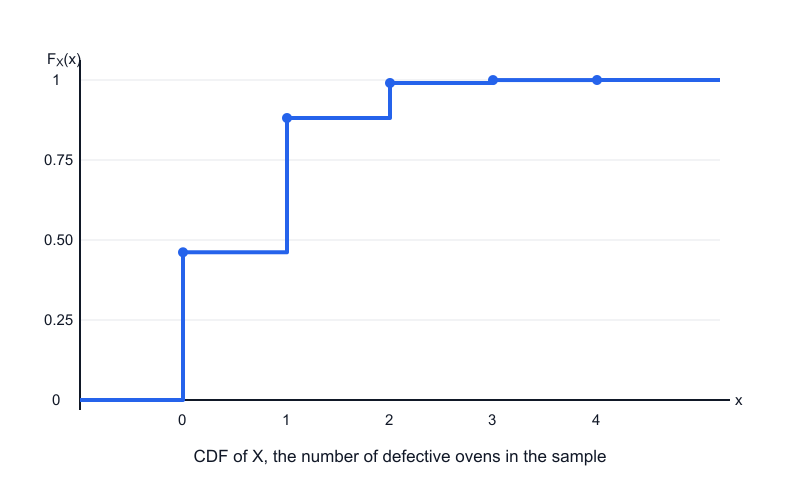
\includegraphics[keepaspectratio,alt={PS1 CB 1.51 CDF}]{assets/fb4e52a015-PS1-CB-1.51-CDF.png}}
\caption{PS1 CB 1.51 CDF}
\end{figure}

\emph{Figure 1. CDF of the number of defective ovens in the sample.}

\subsection{CB 1.53}
\end{quote}

\begin{quote}
\textbf{问题：Problem}

A certain river floods every year. Suppose that the low-water mark is set at \(1\) and the high-water mark \(Y\) has distribution function
\[
F_Y(y)=P(Y\le y)=1-\frac1{y^2},
\qquad 1\le y<\infty.
\]

\begin{enumerate}
\def\labelenumi{(\alph{enumi})}
\item
  Verify that \(F_Y(y)\) is a CDF.
\item
  Find \(f_Y(y)\), the PDF of \(Y\).
\item
  If the low-water mark is reset at \(0\) and we use a unit of measurement that is \(\dfrac1{10}\) of that given previously, the high-water mark becomes \(Z=10(Y-1)\). Find \(F_Z(z)\).
\end{enumerate}
\end{quote}

\begin{quote}
\textbf{解答：Solution}

The complete CDF is

\[
F_Y(y)=
\begin{cases}
0, & y<1,\\[3pt]
1-\dfrac1{y^2}, & y\ge1.
\end{cases}
\]

\subsubsection{(a)}

\(F_Y\) is nondecreasing and right-continuous. In addition,

\[
\begin{aligned}
\lim_{y\to-\infty}F_Y(y)&=0,\\
\lim_{y\to\infty}F_Y(y)&=1.
\end{aligned}
\]

Hence \(F_Y\) satisfies all the conditions of a CDF.

\subsubsection{(b)}

Differentiating the CDF on its continuous part gives

\[
\boxed{
f_Y(y)=
\begin{cases}
\dfrac{2}{y^3}, & y>1,\\[5pt]
0, & y<1.
\end{cases}
}
\]

The value assigned at \(y=1\) is irrelevant for a PDF. Also,

\[
\int_1^\infty \frac{2}{y^3}\,dy=1.
\]

\subsubsection{(c)}

Let \(Z=10(Y-1)\). Since \(Y\ge1\), we have \(Z\ge0\). For \(z\ge0\),

\[
\begin{aligned}
F_Z(z)
&=P\bigl(10(Y-1)\le z\bigr)\\
&=P\left(Y\le1+\frac z{10}\right)\\
&=1-\frac{1}{(1+z/10)^2}\\
&=1-\frac{100}{(z+10)^2}.
\end{aligned}
\]

Therefore,

\[
\boxed{
F_Z(z)=
\begin{cases}
0, & z<0,\\[3pt]
1-\dfrac{100}{(z+10)^2}, & z\ge0.
\end{cases}
}
\]

\subsection{Missiles}
\end{quote}

\begin{quote}
\textbf{问题：Problem}

Suppose we have three missiles: missile 1, missile 2, and missile 3. Suppose each missile is able to hit the enemy plane with probability \(0.7\).

\begin{enumerate}
\def\labelenumi{(\roman{enumi})}
\item
  Without extra information, give a lower bound for the probability of the event ``all missiles hit the enemy plane.''
\item
  If the three missiles are launched independently, what is the probability that the plane is hit?
\end{enumerate}
\end{quote}

\begin{quote}
\textbf{解答：Solution}

Let \(A_i\) be the event that missile \(i\) hits the plane. Then

\[
P(A_i)=0.7,
\qquad
P(A_i^c)=0.3.
\]

\subsubsection{(i)}

Without any assumptions about dependence,

\[
\begin{aligned}
P(A_1\cap A_2\cap A_3)
&=1-P(A_1^c\cup A_2^c\cup A_3^c)\\
&\ge1-\sum_{i=1}^{3}P(A_i^c)\\
&=1-3(0.3).
\end{aligned}
\]

Thus,

\[
\boxed{P(\text{all three hit})\ge0.1}.
\]

\subsubsection{(ii)}

If the missiles operate independently, the plane is hit unless all three missiles miss. Hence

\[
\begin{aligned}
P(\text{plane is hit})
&=1-P(\text{all three miss})\\
&=1-(0.3)^3\\
&=\boxed{0.973}.
\end{aligned}
\]

\subsection{Integer-Valued Random Variable}
\end{quote}

\begin{quote}
\textbf{问题：Problem}

Suppose \(X\) is a random variable taking integer values, \(P(X\ge2)=a\), and \(P(X\le2)=b\). Find \(P(X=2)\) in terms of \(a\) and \(b\).
\end{quote}

\begin{quote}
\textbf{解答：Solution}

Let

\[
A=\{X\ge2\},
\qquad
B=\{X\le2\}.
\]

Then \(A\cup B=S\) and \(A\cap B=\{X=2\}\). By inclusion-exclusion,

\[
\begin{aligned}
1
&=P(A\cup B)\\
&=P(A)+P(B)-P(A\cap B)\\
&=a+b-P(X=2).
\end{aligned}
\]

Therefore,

\[
\boxed{P(X=2)=a+b-1}.
\]

\subsection{Sigma Algebra}
\end{quote}

\begin{quote}
\textbf{问题：Problem}

Consider the random experiment of rolling a die, which gives rise to the sample space
\[
S=\{1,2,3,4,5,6\}.
\]
Let
\[
\mathcal B=\{S,\varnothing,\{1\},\{2\},\{1,2\},\{3,4,5,6\}\}.
\]
Is \(\mathcal B\) a sigma algebra? Explain why.
\end{quote}

\begin{quote}
\textbf{解答：Solution}

The collection

\[
\mathcal B
=\{S,\varnothing,\{1\},\{2\},\{1,2\},\{3,4,5,6\}\}
\]

is not a sigma algebra. For example, \(\{1\}\in\mathcal B\), but its complement is

\[
\{1\}^c=\{2,3,4,5,6\}\notin\mathcal B.
\]

Thus \(\mathcal B\) is not closed under complementation, so

\[
\boxed{\mathcal B\text{ is not a sigma algebra}.}
\]

\subsection{Medical Test}
\end{quote}

\begin{quote}
\textbf{问题：Problem}

Suppose a patient walks into a hospital to get tested for a disease that affects \(1\%\) of the total population. Let \(D\) denote the event that the patient has the disease, and let \(T\) denote the event that the patient's test is positive. Suppose the testing procedure has \(95\%\) sensitivity and specificity:
\[
P(T\mid D)=P(T^c\mid D^c)=0.95.
\]

\begin{enumerate}
\def\labelenumi{(\roman{enumi})}
\item
  Find \(P(D\mid T)\).
\item
  Suppose the proportion of the total population affected by the disease is \(\gamma\) instead of \(1\%\). Find \(P(D\mid T)\) as a function of \(\gamma\). How does it change with \(\gamma\)?
\end{enumerate}
\end{quote}

\begin{quote}
\textbf{解答：Solution}

The test has sensitivity and specificity equal to \(0.95\):

\[
\begin{aligned}
P(T\mid D)&=0.95,\\
P(T\mid D^c)&=1-P(T^c\mid D^c)=0.05.
\end{aligned}
\]

\subsubsection{(i)}

With disease prevalence \(P(D)=0.01\), Bayes' rule gives

\[
\begin{aligned}
P(D\mid T)
&=\frac{P(T\mid D)P(D)}
{P(T\mid D)P(D)+P(T\mid D^c)P(D^c)}\\
&=\frac{0.95(0.01)}
{0.95(0.01)+0.05(0.99)}\\
&=\frac{19}{118}\\
&\approx\boxed{0.1610}.
\end{aligned}
\]

Thus a positive test corresponds to a disease probability of approximately \(16.10\%\).

\subsubsection{(ii)}

If \(P(D)=\gamma\), then

\[
\begin{aligned}
P(D\mid T)
&=\frac{0.95\gamma}
{0.95\gamma+0.05(1-\gamma)}\\
&=\boxed{\frac{19\gamma}{1+18\gamma}}.
\end{aligned}
\]

Moreover,

\[
\frac{d}{d\gamma}
\left(\frac{19\gamma}{1+18\gamma}\right)
=\frac{19}{(1+18\gamma)^2}>0.
\]

Therefore, \(P(D\mid T)\) is strictly increasing in the disease prevalence \(\gamma\).
\end{quote}
